\documentclass[11pt]{article}
\usepackage[margin=1in]{geometry}
\usepackage{graphicx}
\usepackage{booktabs}
\usepackage{xcolor}
\usepackage[labelfont=bf,font=small]{caption}
\usepackage{hyperref}
\hypersetup{colorlinks=true,linkcolor=black,urlcolor=blue}
\graphicspath{{figs/}}
\setlength{\parskip}{0.5em}
\setlength{\parindent}{0pt}

\title{Learning what makes a scaffolded epitope bind:\\
DP4 assay features, models, and how they compare to the composite}
\author{Episcaf v2: DP4 IM0276 readout}
\date{2026-09-22}

\begin{document}
\maketitle

\begin{abstract}
\noindent
The DP4 assay gave us, for the first time, a real binding readout on thousands of designs whose
metrics we already had. This document collects what we learned from it: which features separate
binders from non-binders, which model family predicts binding best, and how a fitted model compares
to the hand-set composite score and Lawson's four-filter. The composite score
was already the right shape (a hand-weighted logistic model), refitting its weights on the assay adds
almost nothing, and the gain comes from adding features of the epitope's own native structure.
The most predictive of those features is rigidity in the bound state. Because that signal disappears
once the antibody is removed, it raises an apo-versus-holo question the static structures cannot settle.
\end{abstract}

\section{The data and what we predict}

The assay is a PepSeq enrichment readout (antibody IM0276 against the DP4 library). We joined it to
the design library on the row-id (\texttt{DP4\_$\langle n\rangle$\_$\langle m\rangle$} $\to$
\texttt{DP4\_$\langle n\rangle$}, 100\% merge). A design counts as a \emph{binder} if it appears in
the assay hit list for its epitope's antibody.

Across the scaffolded arms, 2{,}720 designs carry both a full set of design metrics and an assay call.
Of those, 217 bind, a base rate of 8.0\%. They come from 56 epitopes, each with its own antibody.
That epitope structure matters for how we score every model: we always split by epitope in
cross-validation, so a model is tested on antibodies it never trained on. Scoring within a single
epitope would leak, because the antibody identity, not the design, carries most of the enrichment.

\section{The composite was already a logistic model}

The composite score takes each
design metric, passes it through a saturating sigmoid, multiplies by a hand-set weight, and sums.
Designs that clear all four Lawson filters get a fixed promotion on top. That is the functional
form of a logistic regression with a per-input nonlinearity, and the code says as much
(\texttt{episcaf\_analysis/presets.py}: ``a single-layer perceptron with a per-input nonlinearity and
hand-set weights\ldots to learn the weights instead, fit a logistic regression'').

So fitting a logistic regression is the same object with two changes:
the weights are fit to the assay instead of set from the DP3 prior, and it can take extra inputs. The
ablation below shows which change helped.

\section{Features}

We group the inputs into three blocks (Table~\ref{tab:features}). The design metrics are what we
already compute per design. The secondary-structure counts come from John's per-epitope helix, strand,
and loop tallies. The native-context and dynamics block is new: we read it off each epitope's own
antibody:antigen crystal structure from the RCSB.

\begin{table}[h]
\centering
\caption{The three feature blocks. The native-context block is read from each epitope's deposited
complex with \texttt{biotite}. To locate the epitope inside each complex without guessing chain roles,
we take the antigen chain whose antibody-interface secondary structure best matches John's independent
helix/strand/loop counts; that match also validates the extraction (Pearson $r=0.93$ against John's
helix fraction, MAE $0.10$, $n=56$).}
\label{tab:features}
\small
\begin{tabular}{@{}lll@{}}
\toprule
Block & Features & Source \\
\midrule
Design metrics & cylinder\_clashes, epitope\_rmsd, overall\_rmsd, & pipeline \\
(9) & epitope\_pae, scaffold\_pae, mean\_pae, ptm, & (per design) \\
 & af3\_clashes, island\_index & \\[0.4em]
Secondary & helix, strand, n\_islands & John's counts \\
structure (3) & & (per epitope) \\[0.4em]
Native context & epi\_bfac\_z (bound-state B-factor rigidity), & RCSB complex \\
\& dynamics & epi\_gnm\_apo / \_holo / \_dfit (network-model & (per epitope, \\
 & flexibility, antigen alone vs.\ in complex), & \texttt{biotite}) \\
 & epi\_dsasa (surface buried on binding), & \\
 & epi\_size, epi\_rel\_sasa, epi\_rg, composition & \\
\bottomrule
\end{tabular}
\end{table}

\section{Which features and which model help}

Table~\ref{tab:ablation} and Figure~\ref{fig:ablation} answer both questions at once: we add feature
blocks left to right, and we swap the model family down the rows.

The features drive the result, and the model family matters much less. Fitting a logistic regression on
the same design metrics the composite already uses gives ROC-AUC 0.741, barely above the composite's
0.733. Adding the secondary-structure counts takes it to 0.783, and adding native context and dynamics
takes it to 0.810.

The model family barely matters as long as it is simple. Logistic regression (0.810) and random
forest (0.811) tie at the top with the full feature set, and gradient boosting is close behind (0.796).
The multilayer perceptron is worst at every feature set and actually gets worse as we add features,
which is what a small, noisy dataset does to a model with too many parameters.

\begin{table}[h]
\centering
\caption{Feature ablation crossed with model family. The columns are cumulative: each is the previous
plus one block. \emph{design metrics} (9) are the per-design pipeline outputs (cylinder\_clashes,
epitope\_rmsd, overall\_rmsd, epitope\_pae, scaffold\_pae, mean\_pae, ptm, af3\_clashes, island\_index);
\emph{$+$ secondary structure} adds the epitope's helix, strand, and island counts; \emph{$+$ dynamics}
adds the native-context features epi\_bfac\_z (bound-state rigidity), epi\_gnm\_dfit (change in
flexibility on binding), and epi\_dsasa (surface buried on binding). ROC-AUC under repeated stratified
grouped cross-validation (split by epitope), mean $\pm$ sd over shuffles; composite baseline 0.733.
Adding each block helps every model except the MLP.}
\label{tab:ablation}
\small
\begin{tabular}{@{}lccc@{}}
\toprule
Model & design metrics & $+$ secondary structure & $+$ dynamics \\
\midrule
Logistic regression & $0.741 \pm 0.022$ & $0.783 \pm 0.008$ & $\mathbf{0.810 \pm 0.013}$ \\
Gradient boosting & $0.729 \pm 0.033$ & $0.781 \pm 0.019$ & $0.796 \pm 0.019$ \\
Random forest & $0.720 \pm 0.032$ & $0.791 \pm 0.014$ & $\mathbf{0.811 \pm 0.013}$ \\
MLP (32, 16) & $0.672 \pm 0.024$ & $0.646 \pm 0.014$ & $0.654 \pm 0.013$ \\
\bottomrule
\end{tabular}
\end{table}

\begin{figure}[h]
\centering
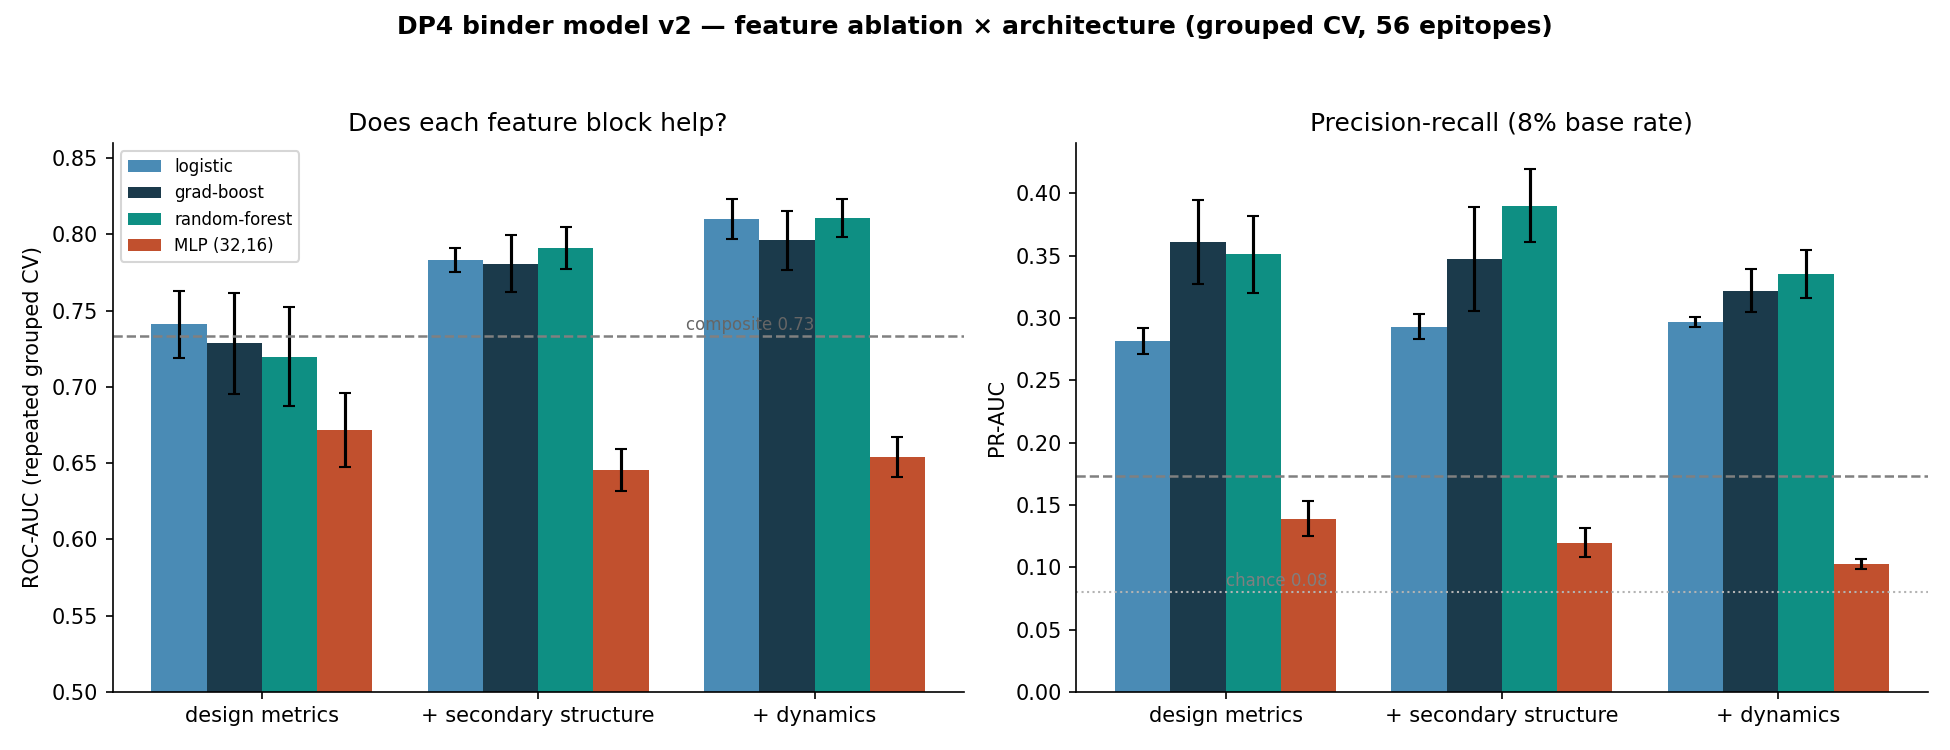
\includegraphics[width=\textwidth]{binder_ml_v2.png}
\caption{\textbf{Feature ablation by model family.} Left: ROC-AUC as we add feature blocks (x-axis),
one bar group per model, error bars over repeated grouped-CV shuffles; the dashed line is the composite
baseline. Right: the same models scored by PR-AUC, which is the fairer view at an 8\% base rate (the
dotted line is chance, 0.08). The pattern is the same in both panels: each feature block lifts the
tree and linear models, the MLP trails, and no model beats a simple one once it has the full feature
set.}
\label{fig:ablation}
\end{figure}

\section{The signal is additive: feature interactions do not help}

The ablation adds feature blocks in one fixed order, so the block added last looks smallest only because
the others are already in. The order-free version is each block's Shapley value: its average marginal
ROC-AUC gain over all orderings of the three blocks, which with three blocks is only eight subsets to
score (Table~\ref{tab:shapley}). Secondary structure is the largest single block, ahead of the nine design
metrics, and on its own it reaches 0.767 of the full model's 0.796. The three values plus the 0.5 baseline
sum to the full-model AUC, so the attribution is exact.

\begin{table}[h]
\centering
\caption{Shapley value of each feature block for gradient boosting: the average marginal ROC-AUC gain over
all orderings of the three blocks (repeated grouped CV). On its own, secondary structure scores 0.767,
design metrics 0.729, dynamics 0.671; the full model is 0.796. The values plus the 0.5 baseline sum to the
full-model AUC, so no block's contribution depends on the order we happen to add it.}
\label{tab:shapley}
\small
\begin{tabular}{@{}lc@{}}
\toprule
Feature block & Shapley value (avg.\ marginal ROC-AUC) \\
\midrule
Secondary structure (helix, strand, island count) & $+0.128$ \\
Design metrics (9) & $+0.109$ \\
Dynamics (rigidity, $\Delta$flex, $\Delta$SASA) & $+0.059$ \\
\midrule
sum $+\ 0.5$ & $0.796$ (= full-model AUC) \\
\bottomrule
\end{tabular}
\end{table}

Shapley still \emph{adds} the blocks; it does not ask whether \emph{combining} features beats adding them.
We test that directly. The gradient booster can be constrained to forbid all cross-feature interactions,
which leaves a purely additive model that is still nonlinear in each feature. Sweeping tree depth with
interactions forbidden versus allowed (Table~\ref{tab:interactions}), the additive model is as good or
better at every depth, and the best model of all is depth-1 stumps, where each tree uses a single feature
and no interaction is possible. The lift over plain logistic regression (0.809 to 0.846) comes entirely
from letting each feature take a nonlinear shape, not from interactions.

\begin{table}[h]
\centering
\caption{Do feature interactions help? ROC-AUC (repeated grouped CV) as tree depth grows, with
cross-feature interactions forbidden (a purely additive model) versus allowed, at matched per-feature
flexibility. Logistic regression (linear and additive) scores 0.809. Forbidding interactions never costs
and usually helps; the best model is depth-1 stumps, additive and nonlinear.}
\label{tab:interactions}
\small
\begin{tabular}{@{}ccc@{}}
\toprule
max tree depth & interactions forbidden (additive) & interactions allowed \\
\midrule
1 & $\mathbf{0.846}$ & $0.846$ \\
2 & $0.838$ & $0.822$ \\
3 & $0.821$ & $0.805$ \\
4 & $0.794$ & $0.793$ \\
6 & $0.786$ & $0.783$ \\
8 & $0.769$ & $0.783$ \\
\bottomrule
\end{tabular}
\end{table}

An Explainable Boosting Machine, a glassbox additive model that adds only the pairwise interactions that
earn their place, confirms this from the other direction: additive-only scores 0.834, and adding up to ten
pairwise interactions drops it to 0.829. Those interaction terms carry 11\% of the model's importance
measured in-sample, yet they lower the held-out AUC. That is a useful reminder in itself: interaction
importance read off the training data is usually overfitting, and only grouped-CV generalization counts.
The EBM's largest main effects are secondary structure (strand and helix), the same conclusion the Shapley
analysis reached.

Figure~\ref{fig:shapes} shows the per-feature response the additive model learns. Read each curve on its
own and add them up; the model's output is the sum of these fifteen shapes. They are gentle bends, not
steps or spikes, which is why a mildly nonlinear additive model captures the signal while a deeper,
interacting one only overfits.

\begin{figure}[h]
\centering
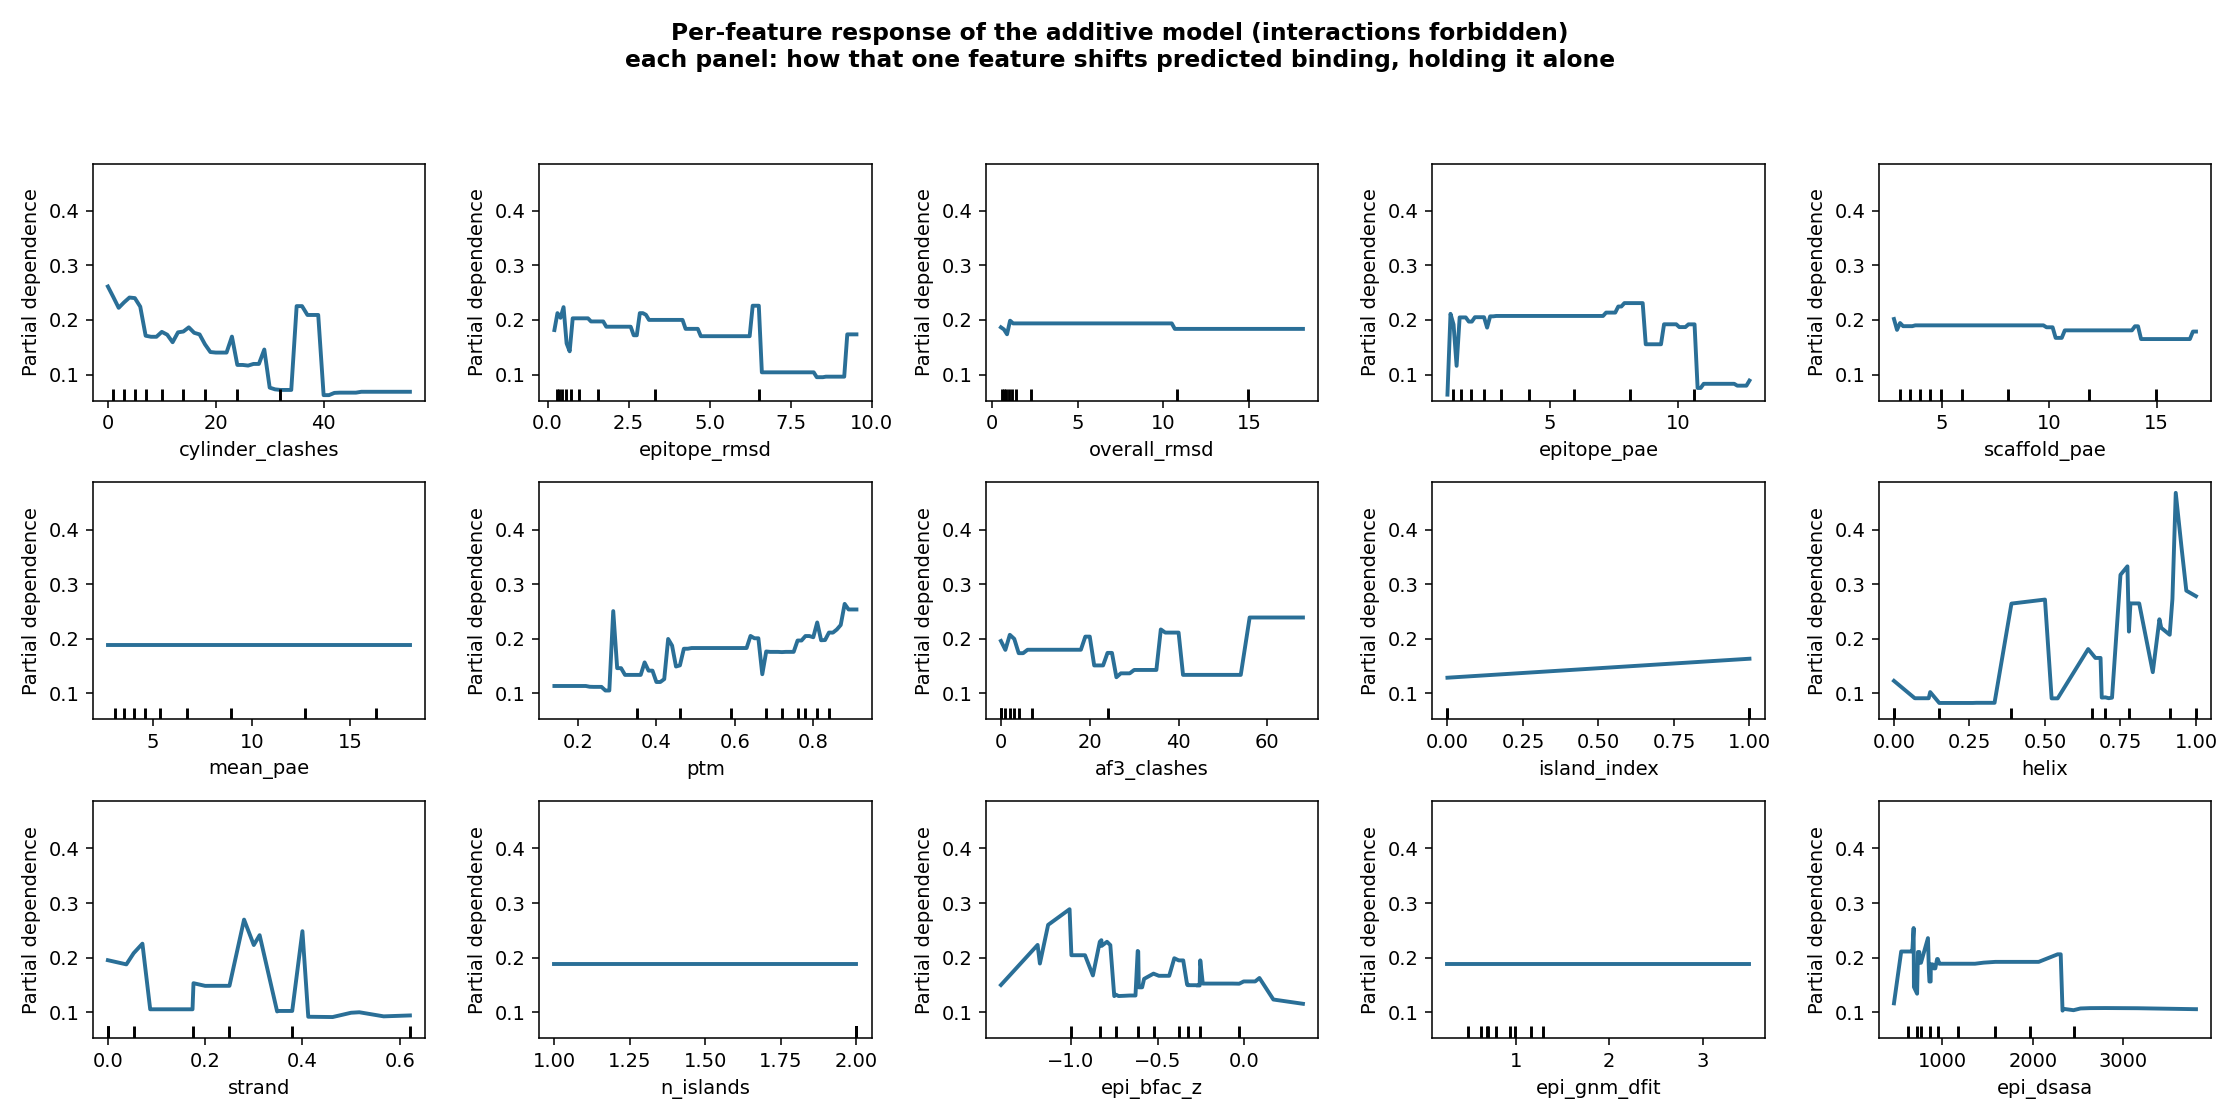
\includegraphics[width=\textwidth]{additive_shapes.png}
\caption{\textbf{Per-feature response of the additive model.} Each panel is one feature's learned
contribution to predicted binding, with interactions forbidden, so the model's score is the sum of these
fifteen curves. The bends are why the additive-nonlinear model beats linear logistic; their mildness is
why adding interactions does not help.}
\label{fig:shapes}
\end{figure}

Together these say the binding signal is an additive, mildly nonlinear scorecard dominated by the
epitope's secondary structure, with no feature interactions that survive out-of-fold. The useful model is
interpretable rather than a black box, and this vindicates the additive form of the composite. One caveat:
at 56 epitopes a subtle real interaction could sit below detection, so this is ``no interaction we can
measure,'' not ``none exists.''

\section{Does any model overfit, and which generalizes best?}

A single held-out split of twelve epitopes is too noisy to rank models, so we repeat it: 20 random
diverse splits, each starting farthest-point sampling from a different seed, each holding out 6 binder
and 6 non-binder epitopes (median 53 test binders per split), with the same feature set as the modeling
section. Table~\ref{tab:headtohead} and Figure~\ref{fig:headtohead} report train and held-out AUC as
mean $\pm$ sd over the splits.

Overfitting shows up as the gap between train and held-out AUC. The oversized MLP has the largest gap
(train 0.995, held-out 0.776, gap 0.219), and its held-out AUC is no better than a plain logistic
regression despite far more parameters. The composite, which is never fit, has no gap at all, with
held-out AUC slightly above train. On unseen diverse epitopes the fitted models cluster between 0.76 and 0.80. Gradient boosting has
the best mean and the lowest variance ($0.796 \pm 0.030$), but the spreads overlap, so the differences
among gradient boosting, random forest, logistic, and the composite are within about one standard
deviation. The small MLP is the one clear laggard ($0.652$).

The repetition also settles the question a single split had raised. On one split logistic looked much
worse than the trees, but that was a small test set and a mismatched feature set. Repeated with the same
features, logistic recovers to $0.757 \pm 0.029$, within a standard deviation of the trees. That is
consistent with the cross-validation in Table~\ref{tab:ablation}: simple models and trees are close, the
MLPs do not help, and the unfit composite is competitive. The two tables differ only in that
Table~\ref{tab:ablation} tests on representative random folds while this one tests on deliberately
diverse, harder epitopes, which is why the held-out numbers here sit a little lower.

\begin{table}[h]
\centering
\caption{Repeated held-out head-to-head: mean $\pm$ sd over 20 random diverse splits (6 binder $+$ 6
non-binder epitopes each, same features as Table~\ref{tab:ablation}). A large train-minus-held-out gap
is overfitting. The oversized MLP has the largest gap and no held-out gain over logistic; the unfit
composite has no gap. On held-out epitopes the fitted models cluster within about one standard
deviation, gradient boosting best in mean and variance.}
\label{tab:headtohead}
\small
\begin{tabular}{@{}lccc@{}}
\toprule
Model & train AUC & held-out AUC & gap \\
\midrule
Composite (no fit) & $0.724 \pm 0.014$ & $0.773 \pm 0.051$ & $-0.049$ \\
Logistic regression & $0.905 \pm 0.008$ & $0.757 \pm 0.029$ & $+0.148$ \\
Gradient boosting & $0.996 \pm 0.001$ & $\mathbf{0.796 \pm 0.030}$ & $+0.201$ \\
Random forest & $0.981 \pm 0.002$ & $0.766 \pm 0.046$ & $+0.215$ \\
MLP (right-sized) & $0.695 \pm 0.024$ & $0.652 \pm 0.070$ & $+0.043$ \\
MLP (oversized) & $0.995 \pm 0.002$ & $0.776 \pm 0.048$ & $+0.219$ \\
\bottomrule
\end{tabular}
\end{table}

\begin{figure}[h]
\centering
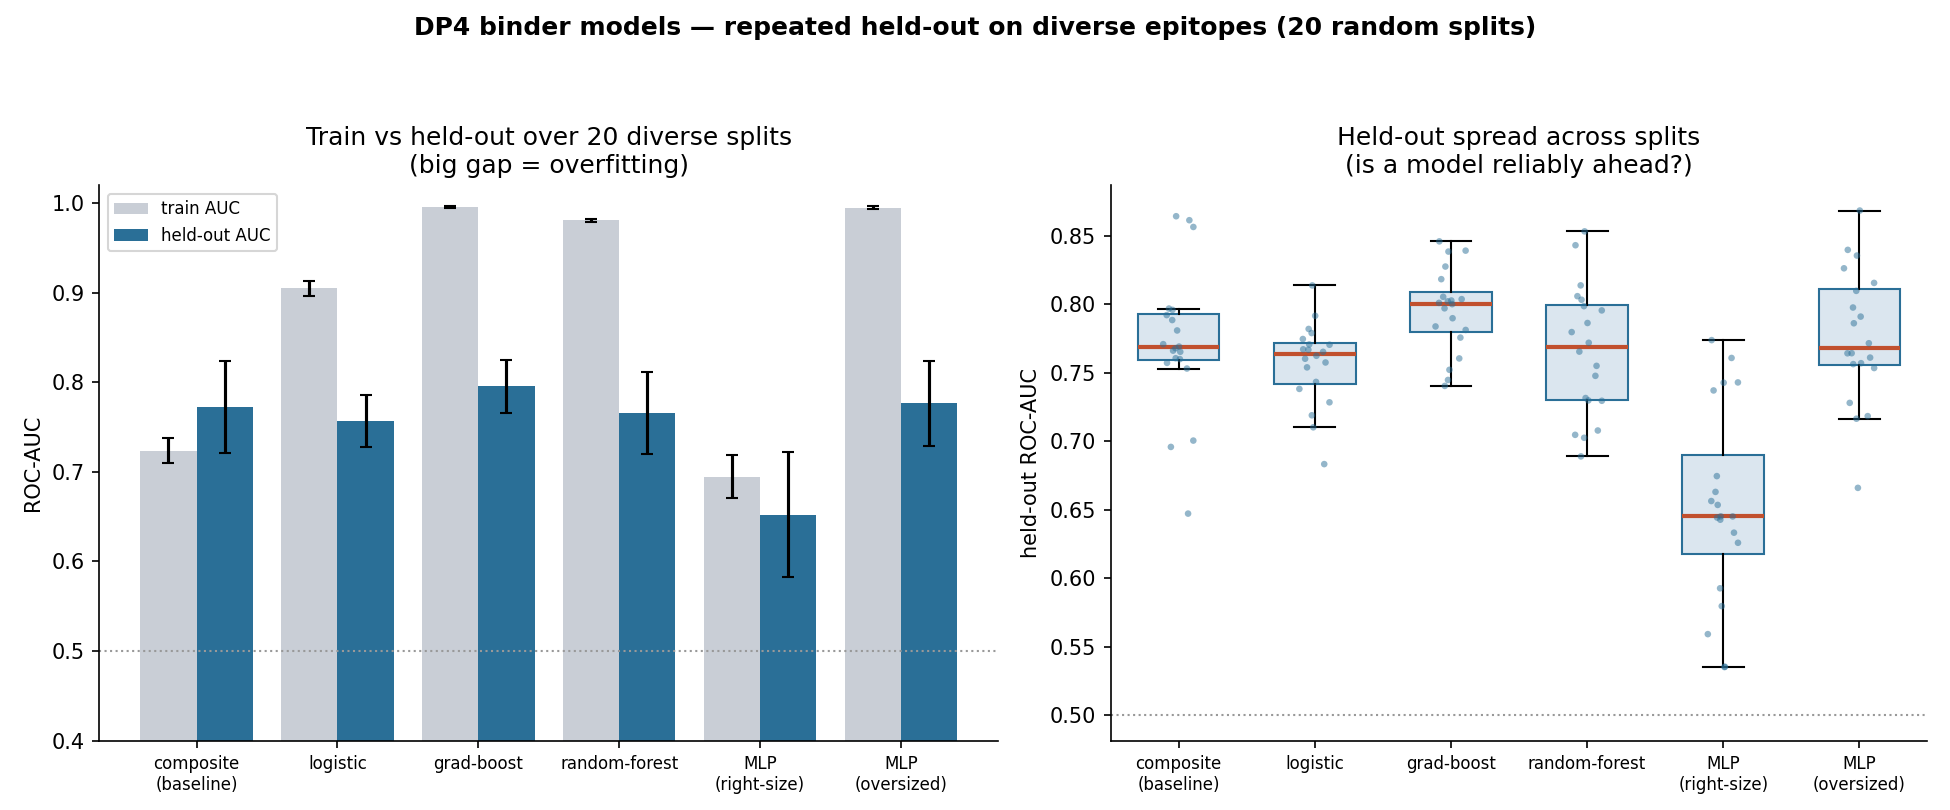
\includegraphics[width=\textwidth]{headtohead.png}
\caption{\textbf{Repeated held-out over 20 diverse splits.} Left: train (grey) and held-out (blue)
ROC-AUC, mean $\pm$ sd across splits; the taller the drop from grey to blue, the more the model overfits.
The oversized MLP has the largest drop and no held-out advantage over logistic, while the unfit composite
does not drop at all. Right: the spread of held-out AUC across the 20 splits for each model (box =
quartiles, red line = median, dots = individual splits). The fitted models overlap heavily between 0.75
and 0.80, so no single one is reliably ahead; the small MLP is the clear laggard.}
\label{fig:headtohead}
\end{figure}

\section{Binary label beats a pseudo-affinity target}

We also asked whether training on a graded target does better than a yes/no label. From the assay
dilution series we built a pseudo-affinity per design (a titration score standing in for $\Delta G$,
since $\Delta G = RT\ln K_d$ is a monotone transform of $K_d$). On the 2{,}412 designs of the 25
antibodies with a usable dilution series, a classifier trained on the binary hit label ranks binders
slightly better than a regressor trained on the pseudo-affinity (ROC-AUC 0.665 vs 0.633,
Figure~\ref{fig:target}). The regressor barely recovers the graded affinity at all
(Spearman between prediction and pseudo-affinity is $-0.10$). Graded affinity, in this readout, is
close to unpredictable from our features; the binary in-or-out question is the one the data can answer.

\begin{figure}[h]
\centering
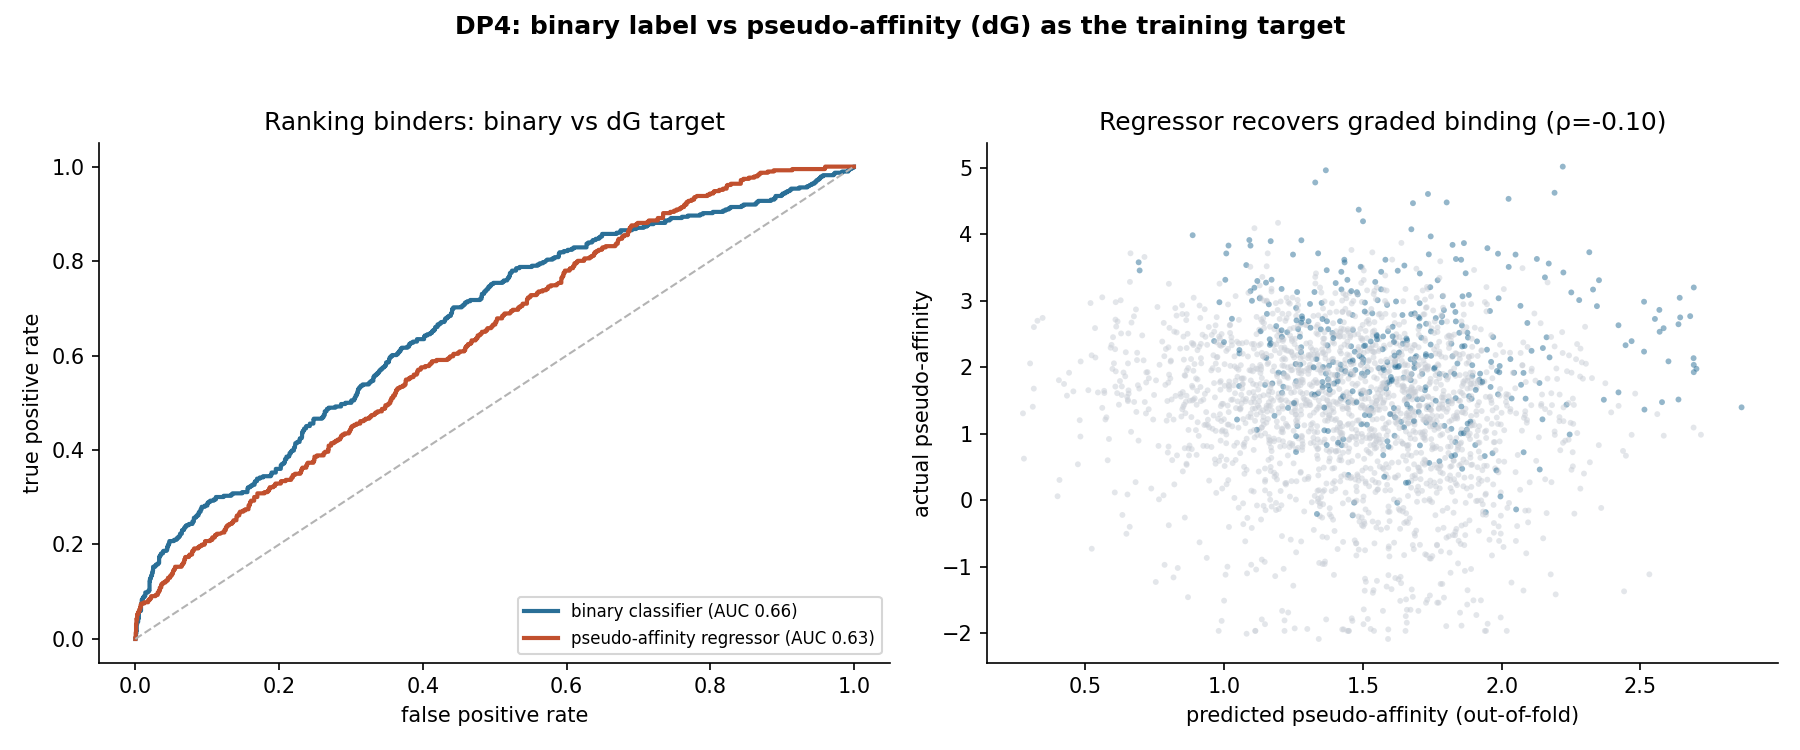
\includegraphics[width=\textwidth]{target_compare.png}
\caption{\textbf{Binary label versus pseudo-affinity as the training target.} Left: ROC for ranking
binders, binary classifier versus pseudo-affinity regressor, same designs and same grouped CV; the
binary target wins. Right: the regressor's predicted pseudo-affinity against the measured value, with
binders highlighted; the cloud is nearly flat, so the graded signal is not there to be learned. We
train on the binary label from here on.}
\label{fig:target}
\end{figure}

\section{The strongest new feature is rigidity in the bound state}

Comparing the 21 binding epitopes to the 35 non-binding ones on the native-context features shows the
largest separation of any feature we tested. Binders sit at lower bound-state B-factor (median
z-score $-0.79$ vs $-0.33$, Mann-Whitney $p<0.001$): the epitopes that scaffold well are the rigid ones
in the crystal. The network-model flexibility of the epitope inside the complex tells the same story
($p=0.001$). Binders also bury less surface on binding (median $\Delta$SASA 891 vs 1255~\AA$^2$,
$p=0.010$), consistent with a pre-formed epitope that does not have to reshape a large interface.

The caveat is what does \emph{not} separate. The apo network-model flexibility, computed with
the antibody removed, does not distinguish binders from non-binders at all (median 0.20 vs 0.27,
$p=0.76$). Every rigidity signal that works is measured in the bound state, where the antibody is
already holding the epitope in place. So we cannot yet tell whether binders are intrinsically
pre-organized before the antibody arrives, or whether they only look rigid because they are clamped.
This is the apo-versus-holo question the v3 simulations are set up to answer, and it is a
concrete reason to run apo dynamics on these epitopes, since the static structures cannot separate the
two cases.

\section{The right way to scaffold depends on the epitope}

Brandon's standing hypothesis was that there is no single rule for good scaffolding, and that the right
metric to optimize depends on the epitope's native context. Figure~\ref{fig:context} tests this
directly. For each design metric we take its within-antibody correlation with binding (the honest
design-level signal, with the antibody effect removed), computed separately inside each context.

The composite predicts binding for helical epitopes (within-antibody correlation $+0.23$) and not at
all for loopy ones ($+0.03$). Accessibility (cylinder\_clashes) predicts strongly for rigid and helical
epitopes ($-0.22$) and weakly for flexible ones ($-0.08$). The AF3 clash term even flips sign between
helical ($-0.19$) and loopy ($+0.04$) epitopes. The design metrics work where the epitope is structured
and rigid, and they lose their grip where it is loopy and flexible. This supports the hypothesis: the
scaffolding rule is context-dependent, so a context-aware model fits the data better than one global rule.

\begin{figure}[h]
\centering
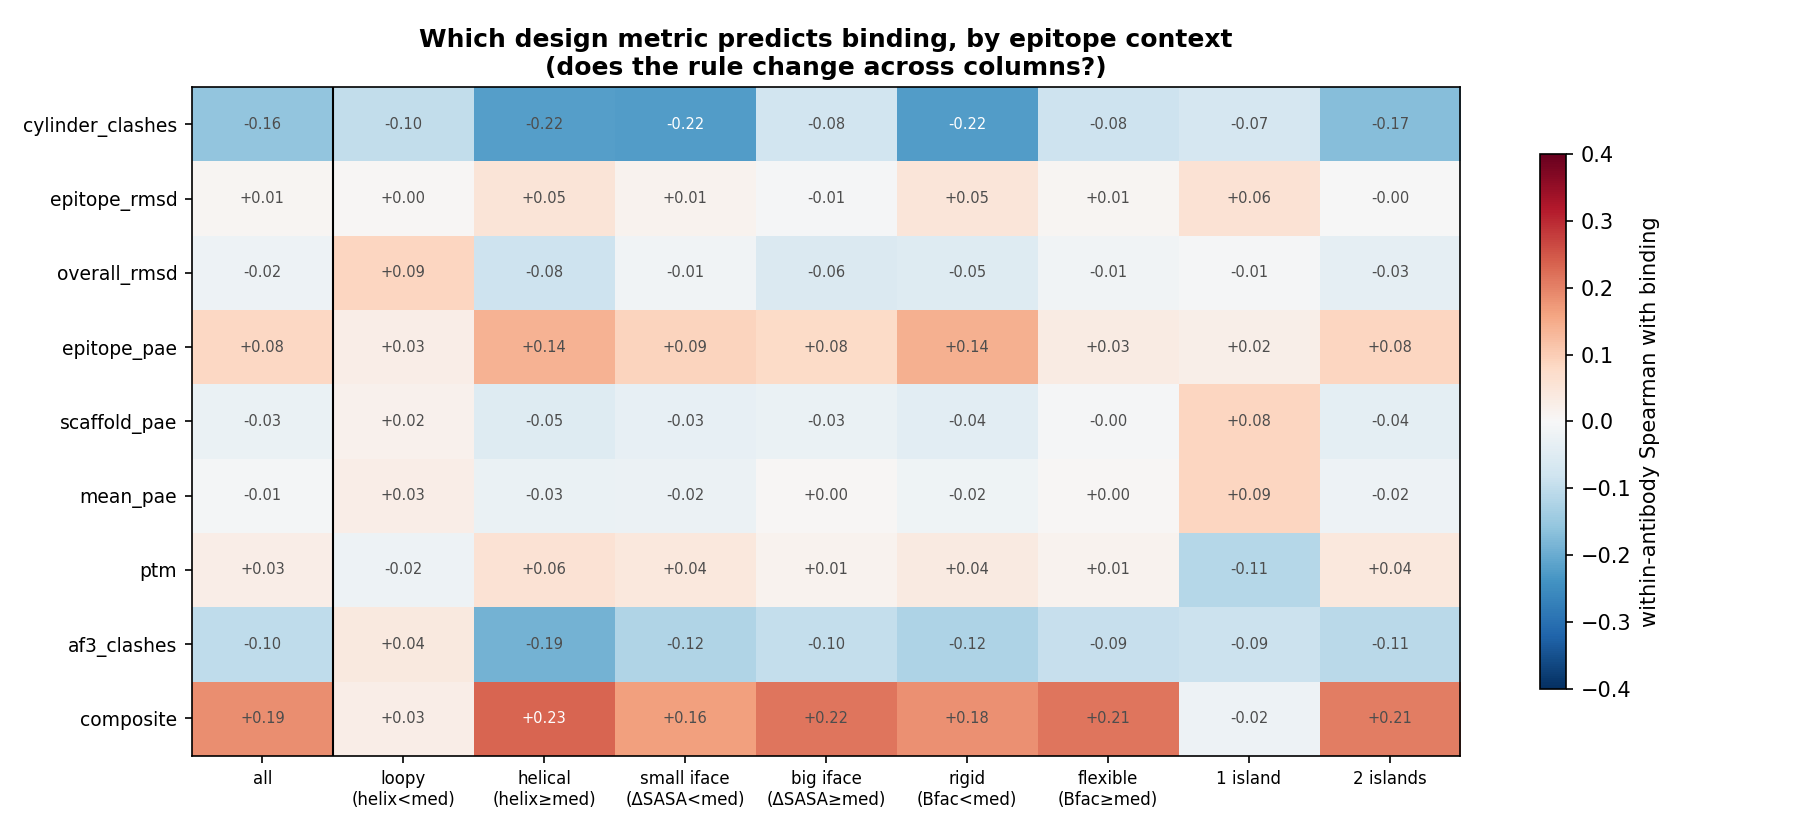
\includegraphics[width=\textwidth]{context_rules.png}
\caption{\textbf{Which design metric predicts binding, by epitope context.} Each cell is the
within-antibody correlation between a design metric (rows) and binding, computed inside one context
stratum (columns); blue means lower metric goes with more binding, the expected direction for clashes
and RMSD. Reading across a row shows whether a metric's usefulness changes with context. The clash and
composite rows change sharply between helical/rigid columns and loopy/flexible ones, which is what a
context-dependent scaffolding rule looks like.}
\label{fig:context}
\end{figure}

\section{How the models compare to the composite and the four-filter}

As a tool for deciding which designs to make, how do the fitted models compare to the composite and to
Lawson's four-filter? We rank designs by each score and screen from the top down. The composite and the
fitted models each give a continuous score, so each traces a curve; the four-filter is a yes/no rule, so
it gives a single operating point. We show both model families, logistic regression and gradient boosting,
each with design metrics only and with the full feature set, so the plots show the model choice and what
the features add at the same time.

Figure~\ref{fig:gain} reads as ``screen the top X\% of designs, catch Y\% of the binders.'' At the top
20\%, the composite catches 44\% of the binders, logistic with all features 60\%, gradient boosting with
all features 67\%, and random picking 20\%. The features help gradient boosting the most: its top-20\%
capture rises from 58\% with design metrics only to 67\% with the full set. For logistic the features show
up more in overall AUC than at the very top of the ranking. The four-filter passes 13\% of designs and
catches 39\% of the binders, an elbow that sits on the composite curve, because the composite's global-pass
promotion is a soft version of the same four filters.

Figure~\ref{fig:roc} is the same comparison as ROC curves. Adding the native-context features lifts both
families by about 0.06 AUC (logistic 0.76 to 0.82, gradient boosting 0.76 to 0.83), and with the full set
the two are within 0.01 of each other. Every fitted curve passes above and to the left of both the
composite curve (AUC 0.73) and the four-filter point (false positive rate 0.11, true positive rate 0.39),
so the fitted scores beat both hand-set rules.

One caveat on this comparison. The models are scored out-of-fold on unseen epitopes, which is fair, but
the composite and the four-filter are the rules that built this library in the first place and were never
fit to this assay. So the fair reading is that the learned weighting beats the hand-set one, and it is
context-aware where the hand-set rule is not. The gap between logistic and gradient boosting is within the
spread we saw in the held-out test (Table~\ref{tab:headtohead}), so we do not read a winner between them.

\begin{figure}[h]
\centering
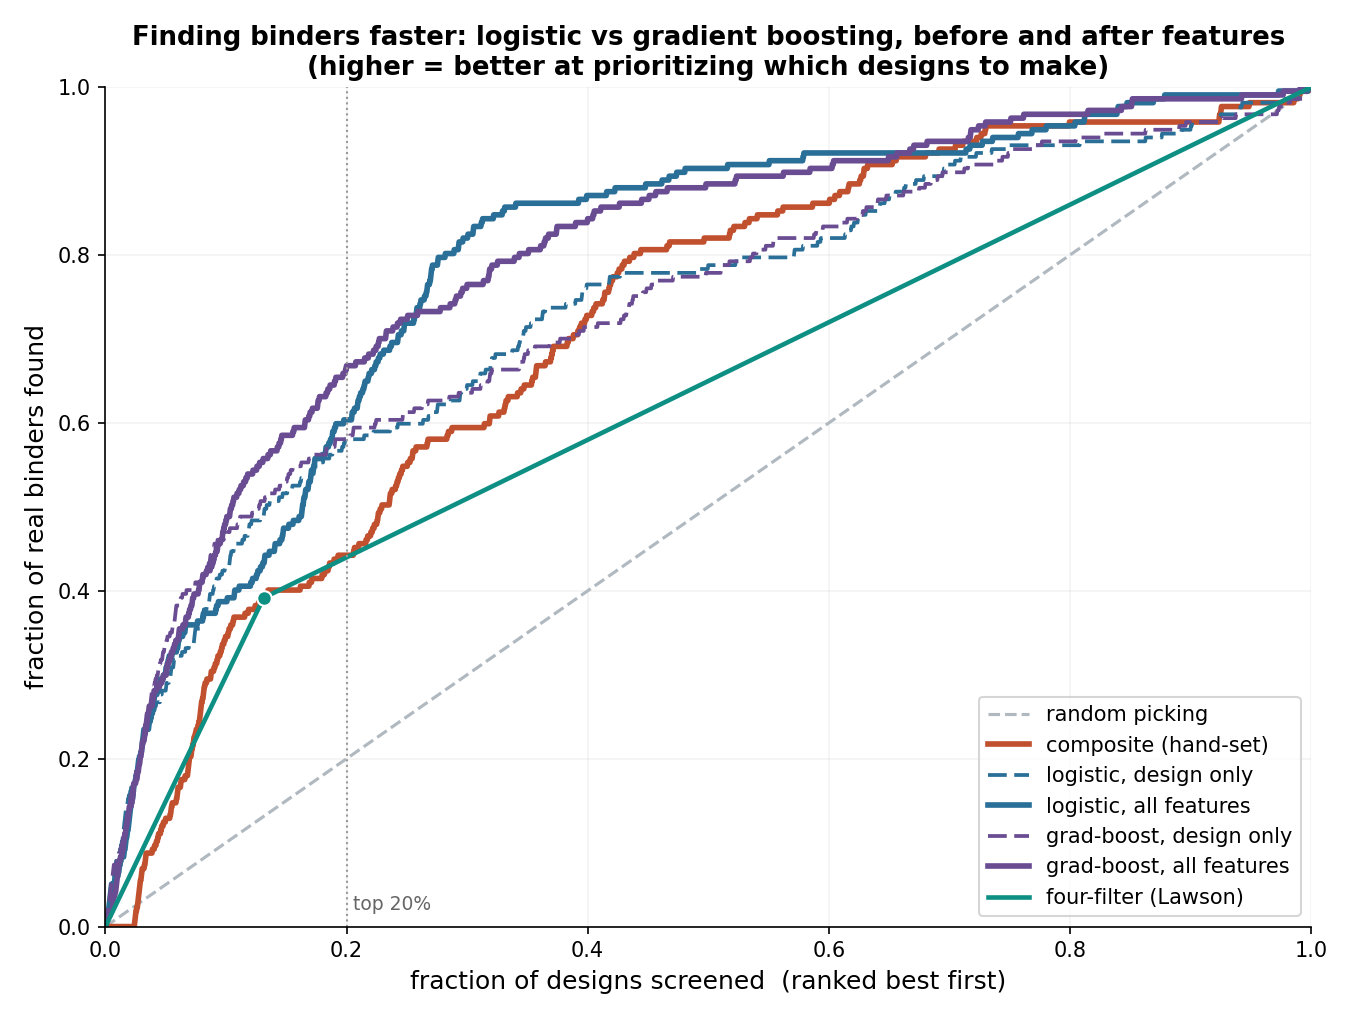
\includegraphics[width=0.86\textwidth]{model_vs_composite.png}
\caption{\textbf{Finding binders faster than the composite.} Rank all designs best-first by each score and
track the fraction of real binders found as you screen deeper (x-axis); higher is better. Two model
families (logistic in blue, gradient boosting in purple) are each shown with design metrics only (dashed)
and the full feature set (solid), against the composite (orange) and random picking (diagonal). The
four-filter (green) is a pass/fail set with no ranking inside it, so its honest gain is two straight
segments through one elbow: make the 13\% of designs that pass, catch 39\% of the binders. At the top
20\% (dotted line) the full-feature models catch the most, gradient boosting the most of all.}
\label{fig:gain}
\end{figure}

\begin{figure}[h]
\centering
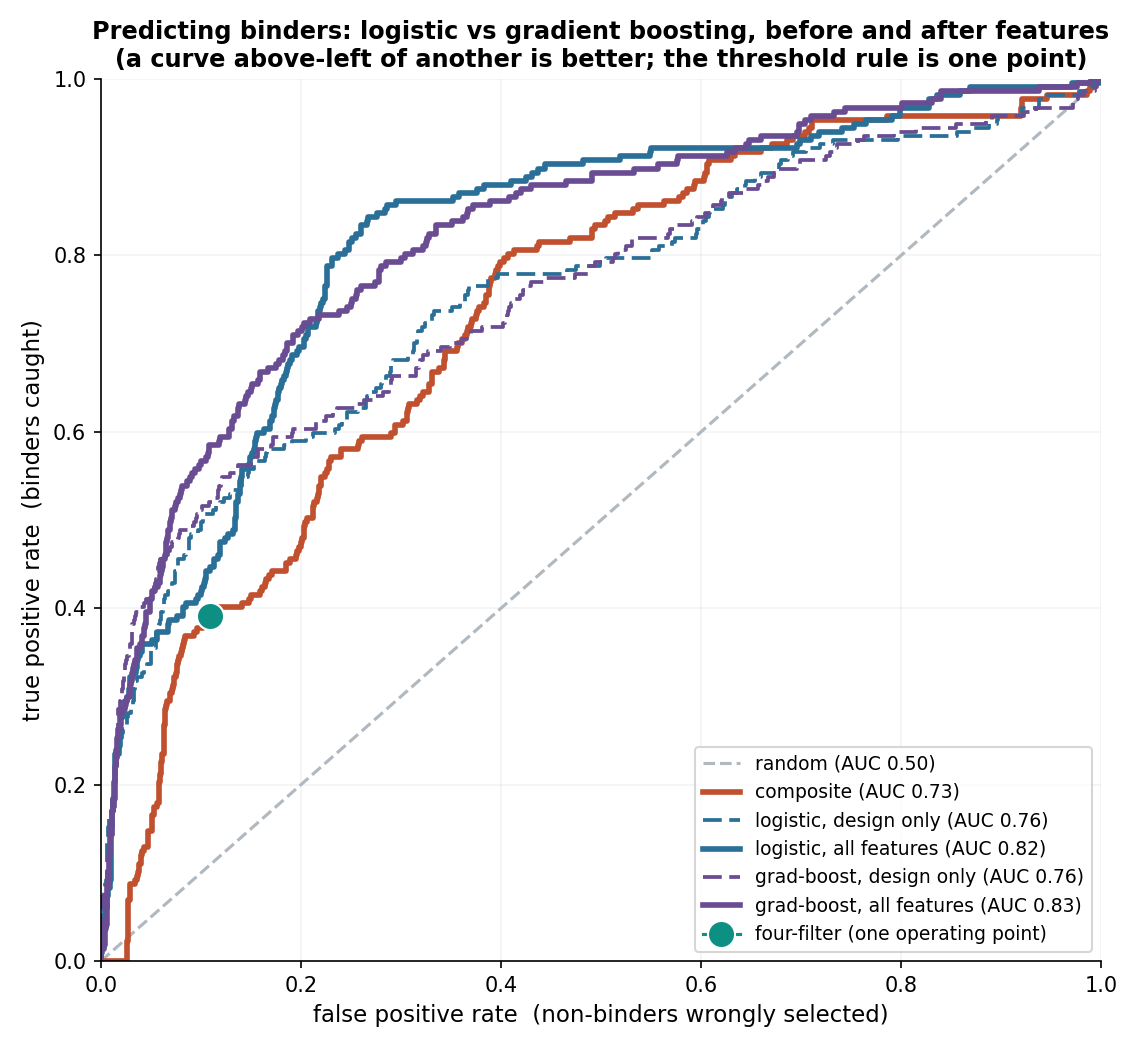
\includegraphics[width=0.72\textwidth]{roc_comparison.png}
\caption{\textbf{Predicting binders: model family and features, as ROC curves.} Same binding truth for
all. Each fitted score sweeps a curve (logistic blue, gradient boosting purple; dashed = design metrics
only, solid = full feature set); the composite is orange and the four-filter is one point (false positive
rate 0.11, true positive rate 0.39). Adding the native-context features lifts both families by about 0.06
AUC, and with the full set logistic (0.82) and gradient boosting (0.83) are within 0.01. Every fitted
curve passes above and to the left of the composite (0.73) and the four-filter point, so the fitted scores
beat both hand-set rules.}
\label{fig:roc}
\end{figure}

\section{Summary and next step}

The composite score was close to the right form already; it is a hand-set version of the model
we can now fit. Refitting its weights on real binding barely helps on its own. The help comes from
giving the model features of the epitope's native structure: its secondary structure carries the
largest single share of the signal, and among the dynamics features, rigidity in the bound state
separates binders most. The best model is additive and interpretable: feature interactions add
nothing that survives out-of-fold, so a per-feature scorecard captures the signal. Because the
rigidity signal disappears when we remove the antibody and look at the epitope alone, we cannot yet
separate ``intrinsically pre-organized'' from ``clamped by the antibody'' with static structures.
Apo dynamics would settle it, and that is the same apo-versus-holo question the v3 campaign already
exists to answer.

One caution applies throughout. 56 epitopes is a small sample for epitope-level features,
every learned model shows a train-test gap, and graded affinity is close to unpredictable here. The
binary in-or-out question is the one this readout can answer, and a simple context-aware model answers it
better than the hand-set rule.

\section*{Reproducibility}

Every number and figure here comes from a named script in \texttt{scripts/}, run on the joined assay
data under \texttt{data/dp4\_binding/}. Structural features need the \texttt{biotite} environment
(\texttt{numpy<2}); the rest run under the repo's Python.

\footnotesize
\begin{tabular}{@{}lll@{}}
\toprule
Script & Produces & Figure \\
\midrule
\texttt{dp4\_im0276\_join.py} & assay-to-library join & (none) \\
\texttt{dp4\_epitope\_features.py} & native-context features & (none) \\
\texttt{dp4\_composite\_vs\_binding.py} & composite vs binding & composite\_vs\_binding.png \\
\texttt{dp4\_binder\_ml\_v2.py} & ablation $\times$ architecture & binder\_ml\_v2.png \\
\texttt{dp4\_feature\_shapley.py} & feature-block Shapley values & (none) \\
\texttt{dp4\_interaction\_test.py} & additive vs interactions, shapes & additive\_shapes.png \\
\texttt{dp4\_ebm.py} & EBM interaction check (needs \texttt{interpret}) & (none) \\
\texttt{dp4\_headtohead.py} & held-out overfitting check & headtohead.png \\
\texttt{dp4\_target\_compare.py} & binary vs pseudo-affinity & target\_compare.png \\
\texttt{dp4\_context\_rules.py} & context-dependent rules & context\_rules.png \\
\texttt{dp4\_model\_vs\_composite.py} & gain curve and ROC & model\_vs\_composite.png, roc\_comparison.png \\
\bottomrule
\end{tabular}

\end{document}
